
Previously, the only way to study ancient animals, plants, and other species was by studying their fossils. This changed in the middle of the 1980's when the first DNA was recovered from almost 5000 years old ancient mummies, showing that it was indeed possible to extract and sequence ancient DNA \autocite{paaboMolecularCloningAncient1985,paaboPreservationDNAAncient1985}. This discovery, along with a dozen other pushing the boundary for what is scientifically possible with ancient DNA, led to Svante Pääbo being awarded with the Nobel Prize in Physiology or Medicine in 2022 for ``his discoveries concerning the genomes of extinct hominins and human evolution'' \autocite{thenobelassemblyatkarolinskainstitutetNobelPrizePhysiology2022}.

The field of ancient DNA (aDNA) was drastically changed with the invention of the Polymerase Chain Reaction, PCR, method \autocite{mullisSpecificEnzymaticAmplification1986} along with the Next Generation Sequencing technology which revolutionized the speed and throughput of genomic sequencing while decimating the cost \autocite{slatkoOverviewNextGeneration2018}. This technological advance has lead to better understanding of human migration and the genealogical tree of modern humans including the previously unknown human (sub)species; the Denisova hominin \autocite{krauseCompleteMitochondrialDNA2010}.

Leaving the homocentric world view, aDNA also allows for the study of archaic animals. In recent years, the boundary of how old DNA can be sequenced has been severely pushed; in 2013 with the early Middle Pleistocene \qtyrange[range-phrase = --,range-units = single]{560}{780}{\kilo\year\BP} horse \autocite{orlandoRecalibratingEquusEvolution2013} and in 2021 with the million-year-old mammoths \autocite{vandervalkMillionyearoldDNASheds2021}. High-throughput sequencing not only allows for the sequencing of single genomes -- like single humans, animals, or plants -- but also for sequencing of entire communities of organisms, so-called metagenomics. By analysing the DNA in environmental samples, environmental DNA, one can survey the rich plant and animal assemblages of a given area and at a specific time in the past. A new paper published in Nature shows that it is now possible to perform metagenomic sequencing on environmental DNA that is 2 million years old, see \autoref{appendix:kapk}. This is a direct application of the statistical method developed in Paper I, see \autoref{chapter:metadmg}, showing that \metaDMG, the method, can help to push the boundary of what is possible with ancient DNA.

Ancient DNA is difficult to work with since it often contains only a limited amount of biological material due to bad preservation, leading to low endogenous content with high duplication rates, making high-depth sequencing difficult \autocite{renaudAuthenticationAssessmentContamination2019}. Genotype likelihoods are often used to alleviate the problem of low-coverage data \autocite{nielsenGenotypeSNPCalling2011}.
In addition to this, the DNA is often highly degraded. In particular, the two prominent issues with aDNA is fragmentation and deamination \autocite{dabneyAncientDNADamage2013,peyregnePresentDayDNAContamination2020,}. Fragmentation refers to the fact that the DNA is broken into very short fragments, often with a fragment size of less than \SI{50}{\basepairs}. This leads to low-quality mapping issues and reference biases, which can somewhat be mitigated by the use variant graphs \autocite{martinianoRemovingReferenceBias2020}.
Deamination is a process in which cytosine (C) in the single-stranded overhangs in the end of the DNA molecules is often hydrolized to uracil (U) which is then read as thymine (T) by the DNA polymerase. This particular type of postmortem damage is known as cytosine deamination, or C-to-T transitions, and is a one of the main reasons behind nucleotide misincorporations in ancient DNA \autocite{briggsPatternsDamageGenomic2007}. Due to the short fragment sizes in ancient DNA, they will often contain overhangs with over-expressed C-to-T frequency. In the case of single-genome analysis, previous solutions have been to either remove all transitions and only keep transversions, or apply trimming at the read ends \autocite{schubertImprovingAncientDNA2012}.
For an illustration of both fragmentation and deamination of ancient DNA, see  \autoref{fig:dna-damage-overview}.

\begin{figure}[htbp]
    \sidecaption{
        Illustration of DNA damage. Ancient DNA is often highly fragmented with short reads compared to modern, present-day DNA, and can contain uracils (U). These uracils will then be misread as thymines (T) while sequencing leading to C-T nucleotide misincorporations. This is primaryly happening at the end of the reads. Modified from \autocite{peyregnePresentDayDNAContamination2020}.
        \label{fig:dna-damage-overview}}
    \centering
    \includegraphics[trim={0mm 90mm 0mm 90mm}, clip, width=\textwidth]{figures/illustrator/dna-deamination.pdf}
\end{figure}

Currently, a handfull of different methods for quantifying ancient DNA damage exists. In particular, the mapDamage 2.0 software has been the gold standard for how to measure ancient DNA damage in the field \autocite{jonssonMapDamage2FastApproximate2013}, however, it uses slow algorithms leading to unfeasible runtimes for large datasets. Newer, faster methods are being developed all of the time, such as PyDamage \autocite{borryPyDamageAutomatedAncient2021} which tackle some of mapDamage's limitations, although even faster methods suited at metagenomic analysis for large-scale datasets are still lacking.

In Paper I, see \autoref{chapter:metadmg}, we introduce the \metaDMG  software which utilizes the C-to-T deamination pattern\sidenote{for the forward strand and the G-to-A deamination pattern for the reverse strand} to identify ancient DNA damage. One of the key features of this method is the beta-binomial model which allows the uncertainty to fitted independently of the mean leading to improved accuracy of the damage estimation. Since the data is based on misincorporation counts, in particular the number of C-to-T transitions, $k$, out of $N$ total C's, the classical likelihood to use for this type of data is a binomial distribution. The mean and variance of the binomial distribution is given by:
\begin{equation}
    \begin{split}
        \EX{k}  &= N p \\
        \VarX{k} &= Np(1-p),
        \label{eq:Binomial_expectation_variance}
    \end{split}
\end{equation}
where $p$ is the probability of success (a C-to-T substitution). One of the issues, however, is that the variance of the binomial distribution is proportional to the mean. The binomial distribution is thus not flexible enough to accommodate large amounts of variance in the data, so-called overdispersion \autocite{mcelreathStatisticalRethinkingBayesian2020}. One way to accommodate overdispersion is to instead use a beta-binomial model. The beta-binomial model is a generalization of the binomial distribution where the variance is allowed to be flexible. Technically, the beta-binomial model assumes that $p$ is a random variable which follows a beta distribution $p \sim \mathrm{Beta}(\mu, \phi)$ where the beta distribution is parameterized\sidenote{This can be reparameterization in term of the classical $\alpha, \beta$ parameterization by: $\mu = \alpha / (\alpha + \beta)$ and $\phi = \alpha + \beta$.} in terms of its mean, $\mu$, and dispersion parameter, $\phi$, \autocite{cepeda-cuervoDoubleGeneralizedBetaBinomial2017}. The mean and variance of this beta-binomial model is then given by:
\begin{equation}
    \begin{split}
        \EX{k}  &= N \mu \\
        \VarX{k} &= N\mu(1-\mu) \frac{\phi+N}{\phi+1}.
        \label{eq:BetaBinomial_expectation_variance}
    \end{split}
\end{equation}

Comparing \autoref{eq:Binomial_expectation_variance} and \autoref{eq:BetaBinomial_expectation_variance}, we see that the variance of the beta-binomial model is no longer (strictly) proportional to the mean, but instead is a function of the dispersion parameter, $\phi$, allowing for higher variance than the binomial-only model. When $\phi = 0$, the variance of the beta-binomial model is $N$ times larger, and when $\phi \rightarrow \infty$ the variance reduces to the variance of the binomial model, showing that the beta-binomial model is a generalization of the binomial model.

\autoref{eq:BetaBinomial_expectation_variance} shows how we model the C-to-T damage at a specific base position in the read. We model the position-dependent damage frequency, $f(x) = k(x) \ N(x)$, see \autoref{fig:dna-damage-overview}, as a function of the distance from the end of the read, $x$, with an exponential decay:
\begin{align}
    f(x; A, q, c) = A(1-q)^{x-1} + c.
    \label{eq:damage_function}
\end{align}
Here $A$ is the scale factor, or amplitude, $q$ is the decay rate, and $c$ is a constant offset, the baseline damage. Since $x$ is discrete, this is similar to a (modified) geometric sequence starting from $x=1$. The combination of \autoref{eq:BetaBinomial_expectation_variance} and \autoref{eq:damage_function} is illustrated in \autoref{fig:damage-model-sketch}, which shows the position-dependent, decreasing damage frequency. The figure also shows the increase in uncertainty in the beta-binomial model compared to the binomial-only model.
\begin{figure}[htbp]
    \sidecaption{
        Illustration of the damage model. The figure shows data points as circles and the damage frequency, $f(x)$, as a solid line. The amplitude of the damage is $A$, the offset is $c$, and the relative decrease in damage pr. position is given by $q$. The damage uncertainty for a binomial model is shown in dark grey and the uncertainty for a beta-binomial model in light grey.
        \label{fig:damage-model-sketch}}
    \centering
    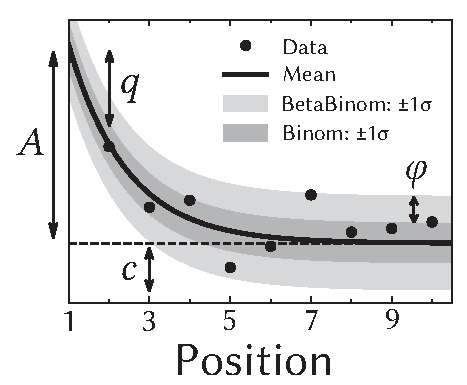
\includegraphics[width=0.6\textwidth]{figures/damage_sketch_new.pdf}
\end{figure}

The damage framework described above is based on the nucleotide misincorporations, i.e. the C-to-T transitions. The background for this data can be from either sequence files (fasta or fastq files) mapped to a single genome or from metagenomic data consisting of multiple mapped reads. As such, the damage framework is a general tool for estimating damage.
In the metagenomic case where single DNA reads are mapped to multiple species, \metaDMG performs a simple lowest common ancestor based on the ngsLCA algorithm \autocite{wangNgsLCAToolkitFasta}. This means that for each read that map to multiple reference, i.e. has multiple alignments, the taxonomic tree is traversed for each alignment until a common ancestor is found. This is the so-called lowest common ancestor (LCA). \autoref{fig:tree-LCA} illustrates the LCA for a read that maps to different (sub)species. In this example, the LCA of alignment 1 and 2 is the Subspecies I while the LCA for all four alignments is the Genus X. \metaDMG works by default with the NCBI taxanomic database but can also be used with custom databases.

\begin{figure}[htbp]
    \sidecaption{
        Illustration of the lowest common ancestor (LCA) for taxonomic trees. Here the LCA of alignment 1 and 2 is Subspecies I, while the LCA of all four reads is Genus X. The dots ($\dots$) refers to other taxonomic levels, e.g. family and order.
        \label{fig:tree-LCA}}
    \centering
    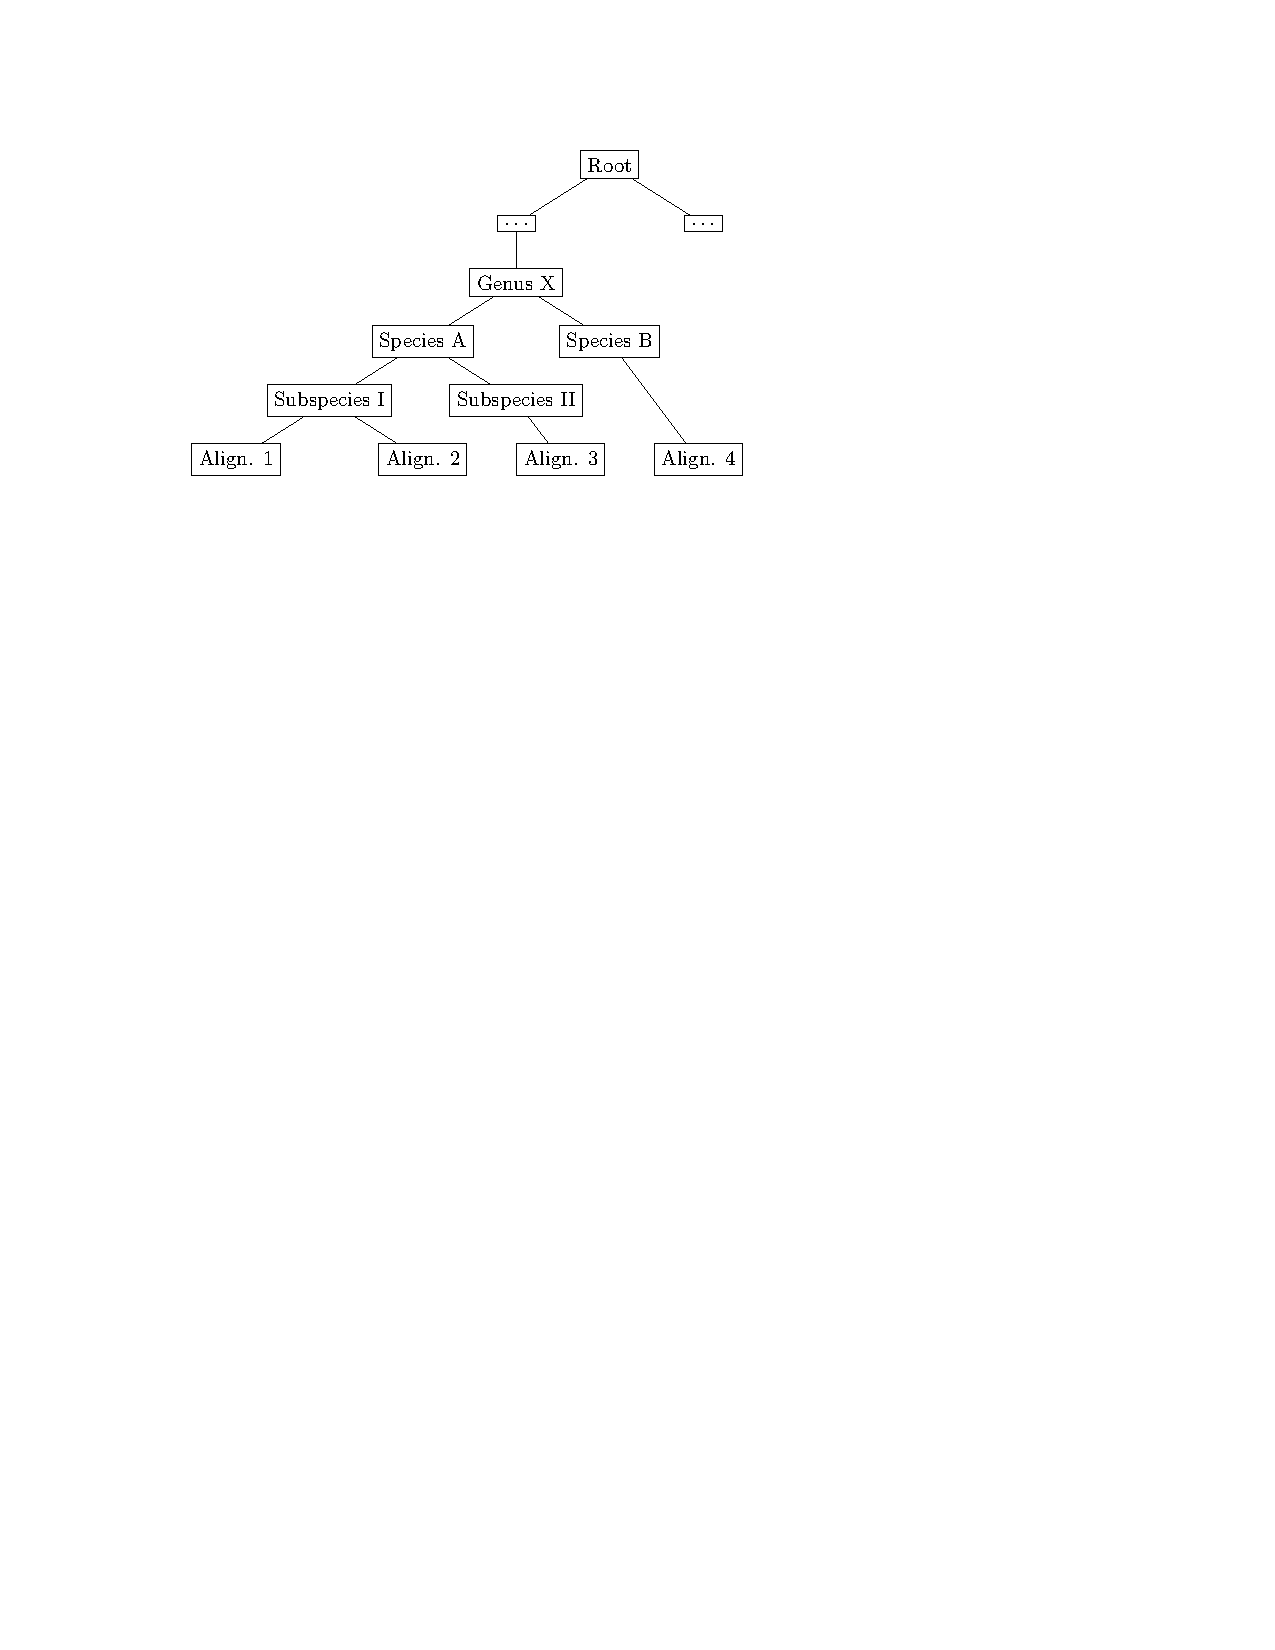
\includegraphics[trim={3cm 19.5cm 8.5cm 2.3cm}, clip,width=0.8\textwidth]{figures/tree.pdf}
\end{figure}

Given the nucleotide misincorporations, either coming from a single-reference alignment file or after LCA in the metagenomic case, we fit eq. \eqref{eq:BetaBinomial_expectation_variance} and \eqref{eq:damage_function} with a Bayesian model. This is done to ensure the optimal inference of the parameters, $A$, $q$, and $c$, and to account for the uncertainty in the data. Bayesian inference also allows for the inclusion of domain knowledge in the form of the prior distribution by Bayes theorem. Bayes theorem is based on the law of conditional probability \autocite{barlowStatisticsGuideUse1993} stating that the probability of two events, $A$ and $B$, both happening, $P(A \cap B)$, is given by the probability of $B$, $P(B)$ times the probability of $A$ given $B$, $P(A|B)$:
\begin{align}
    P(A \cap B) = P(B)P(A|B).
    \label{eq:bayes_theorem_1}
\end{align}
Similarly, $P(A \cap B)$ can also be expressed in terms of the probability of $A$:
\begin{align}
    P(A \cap B) = P(A)P(B|A).
    \label{eq:bayes_theorem_2}
\end{align}
Combining \autoref{eq:bayes_theorem_1} and \autoref{eq:bayes_theorem_2} and rearranging terms gives the Bayes theorem:
\begin{align}
    P(\theta|x) = \frac{P(\theta)P(x|\theta)}{P(x)},
    \label{eq:bayes_theorem}
\end{align}
with a change of variables where $x$ now refers to the observed data and $\theta$ the parameter(s) of the model. The first term in the numerator, $P(\theta)$, is the prior distribution and describes the probability distribution assigned to $\theta$ before observing any data. The second term is the likelihood function, $P(x|\theta)$, which is the probability of observing the data, $x$, given the parameter(s), $\theta$. Together these two terms combine to a compromise between data and prior information.

The numerator, $P(x)$, also known as the evidence, can be treated as a data-related normalization factor. In the case of continuous $\theta$, this can calculated as the marginalization of the likelihood function over $\theta$:
\begin{align}
    P(x) = \int_\theta P(x|\theta)P(\theta) \dx \theta.
    \label{eq:evidence}
\end{align}
This equation, however, is often intractable to compute in the higher-dimensional case. Luckily, it can be shown that Markov Chain Monte Carlo (MCMC) sampling can approximate the posterior distribution, $P(\theta|x)$, and asymptotically converge to the correct distribution \autocite{gelmanBayesianDataAnalysis2015a}.

Traditionally MCMC methods such as Metropolis Hastings (MH) or Gibbs sampling have been used for Bayesian inference, however, these methods are often slow and require a lot of tuning. In the last decades, a new class of MCMC methods have been developed, namely Hamiltonian Monte Carlo (HMC) methods. While traditional MH uses a Gaussian random walk, HMC is a gradient-based MCMC method that uses Hamiltonian dynamics to guide the sampling. This makes HMC more efficient than traditional MCMC methods and allows for sampling from high-dimensional distributions \autocite{betancourtConceptualIntroductionHamiltonian2018,nealMCMCUsingHamiltonian2011}. A particularly efficient variant of HMC is the No-U-Turn Sampler (NUTS). NUTS is a variant of HMC that automatically tunes the step size and number of steps to take in the Hamiltonian dynamics \autocite{homanNoUturnSamplerAdaptively2014}.

Most statistical domain-specific languages (DSL) such as Stan \autocite{carpenter2017stan}, Pyro \autocite{bingham2019pyro}, NumPyro \autocite{phanComposableEffectsFlexible2019} or Turing.jl \autocite{geTuringLanguageFlexible2018}, implement HMC and in particular the NUTS algorithm. Since \metaDMG is implemented in Python, we use NumPyro for the Bayesian inference of the damage model as it is easy to implement and computationally efficient since it which uses JAX \autocite{bradburyJAXComposableTransformations2018} under the hood for automatic differentiation and just-in-time (JIT) compilation.

Even though NumPyro is fast and \metaDMG is efficiently implemented, the Bayesian inference of the damage model is still computationally expensive. Thus, we have decided to also include a faster, approximate method of Bayesian inference: the maximum a posteriori (MAP) estimate. The MAP estimate is the point estimate of the posterior distribution that maximizes the posterior probability density function, i.e. the posterior mode:
\begin{align}
    \hat{\theta}_\mathrm{MAP} = \argmax_\theta P(\theta|x) = \argmax_\theta P(\theta)P(x|\theta),
\end{align}
where the second equality is due to the evidence being independent of $\theta$. Since this is a point estimate, $\hat{\theta}_\mathrm{MAP}$ does not fully explain the full posterior, however, it is often a good approximation\footnote{Especially when the posterior is unimodal, which it generally is in the case of \metaDMG.}. Comparing $\hat{\theta}_\mathrm{MAP}$ to the maximum likelihood estimate (MLE):
\begin{align}
    \hat{\theta}_\mathrm{MLE} = \argmax_\theta P(x|\theta),
\end{align}
the MAP estimate can be seen as a regularized version of the MLE estimate \autocite{10.5555/2380985}. To further optimize the computational efficacy of the MAP estimation in \metaDMG, we JIT compile the MAP estimation function using Numba \autocite{lamNumbaLLVMbasedPython2015} and mathematically optimize the function with iMinuit \autocite{dembinskiScikithepIminuitV22021}.

One of the limitations of the \metaDMG software is XXX.
